\chapter{Planificación}
\thispagestyle{fancy}

\fancyhead[LE]{\thechapter.Planificació} 

La planificación de este proyecto se ha realizado con un diagrama GANTT. Este esta presente en la tabla \ref{table:planificacion}, en caso de querer observar la tabla a una escala mayor esta se encuentra en el Anexo \ref{appendix:Documentos} sección \ref{appendix:Documentos_Planificacion}.
\\ \\
La planificación de este proyecto es un proceso complejo que ha de contener todos los pasos necesarios para conseguir el objetivo del estudio. Para ello se ha dividido en 4 fases de 3 semanas, empezando la primera el 22 de Febrero de 2021 y terminando la ultima fase el 16 de mayo de 2021.
\\ \\
Las tareas de este proyecto se han agrupado en varios grupos:
\begin{itemize}
    \item El registro del proyecto.
    \item La formación.
    \item Configuración del hardware.
    \item Adaptación del RS online a aprendizaje federado.
    \item Desarrollo de la memoria.
    \item Estudio del rendimiento
\end{itemize}
A su vez, estos grupos cuentan con subtareas más concretas que permiten programar adecuadamente la duración del proyecto.
\begin{itemize}
    \item El registro del proyecto. 
        \begin{itemize}
            \item [$\diamond$]Definición de título y descripción.
            \item [$\diamond$]Registro del proyecto a través del formulario.
        \end{itemize}
    \item La formación.
        \begin{itemize}
            \item [$\diamond$]Formación sobre conceptos de Machine Learning.
            \item [$\diamond$]Formación sobre conceptos de los sistemas de recomendación.
            \item [$\diamond$]Formación sobre conceptos de Federated Learning.
            \item [$\diamond$]Formación sobre LightFM.
            \item [$\diamond$]Familiarización con el RS de R.Sánchez.
        \end{itemize}
    \item Configuración del hardware.
        \begin{itemize}
            \item [$\diamond$]Configuración de las RaspBerrys.
            \item [$\diamond$]Configuración de la JetsonNano.
            \item [$\diamond$]Aprovisionamiento de los Sistemas Operativos.
            \item [$\diamond$]Instalar y ejecutar RS.
        \end{itemize}
    \item Adaptación del RS online a aprendizaje federado.
        \begin{itemize}
            \item [$\diamond$]Guardado , cargado y envío de modelos de IA.
            \item [$\diamond$]Agregación de los modelos de IA.
            \item [$\diamond$]Recomendación para un único usuario.
            \item [$\diamond$]Combinar recomendaciones para un único usuario.
            \item [$\diamond$]Combinar recomendaciones para varios usuario.
            \item [$\diamond$]Reentrenar modelos.
            \item [$\diamond$]Visualización de los resultados de rendimiento por gráficas.
        \end{itemize}
    \item Desarrollo de la memoria.
        \begin{itemize}
            \item [$\diamond$]Resumen.
            \item [$\diamond$]Introducción.
            \item [$\diamond$]Antecedentes y Justificación.
            \item [$\diamond$]Objetivos y Alcance.
            \item [$\diamond$]Consideraciones éticas.
            \item [$\diamond$]Metodología.
            \item [$\diamond$]Planificación.
            \item [$\diamond$]Introducción al Federated Learning.
            \item [$\diamond$]Desarrollo.
            \item [$\diamond$]Presupuesto.
            \item [$\diamond$]Conclusiones y Trabajo futuro.
            \item [$\diamond$]Bibliografía.
            \item [$\diamond$]Definiciones y Acrónimos.
            \item [$\diamond$]Anexos.
        \end{itemize}
    \item Estudio del rendimiento.
        \begin{itemize}
            \item [$\diamond$]Estudio del rendimiento de un RS centralizado.
            \item [$\diamond$]Estudio del rendimiento de un RS de modelos agregados.
            \item [$\diamond$]Estudio de rendimiento del sistemas de recomendaciones final.
        \end{itemize}
\end{itemize}
\newpage
\begin{table}
    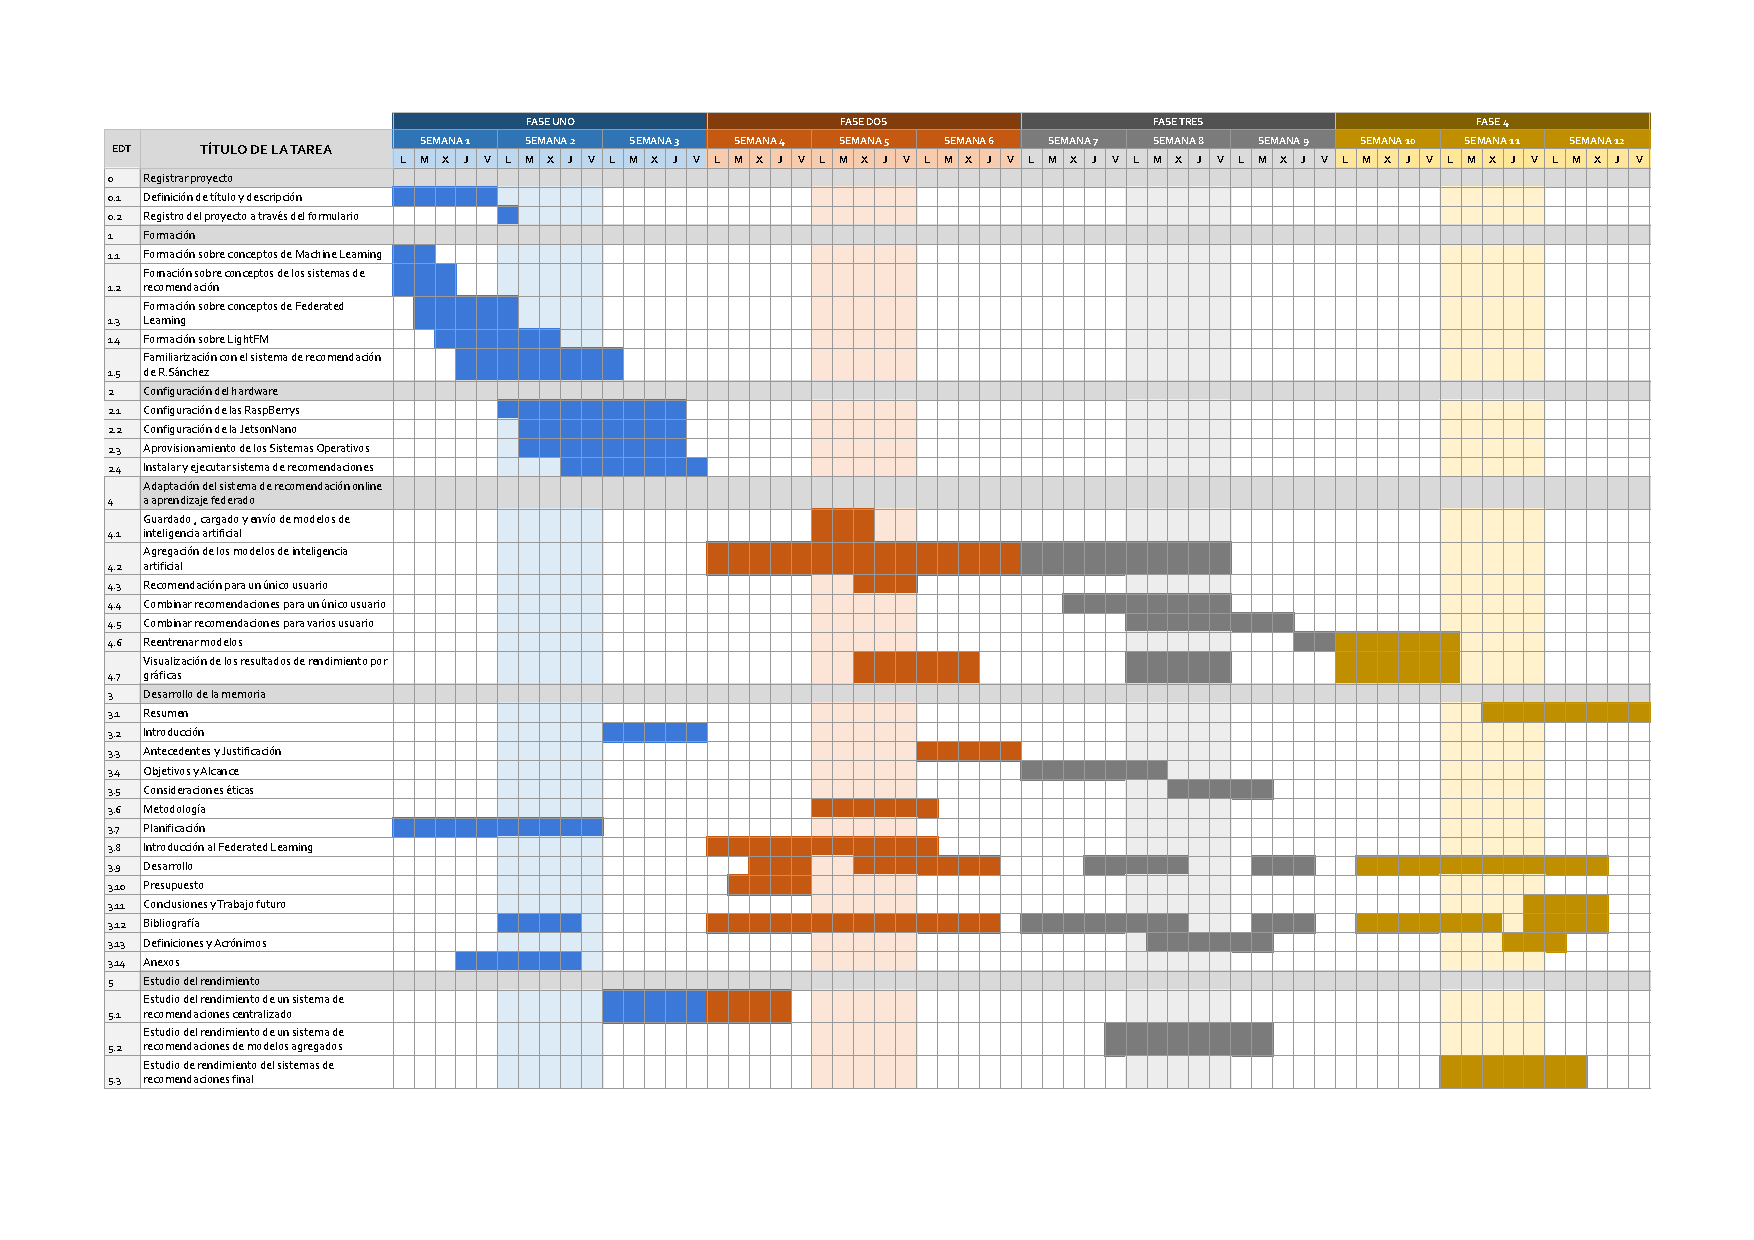
\includegraphics[angle=90,  width=\linewidth, height=\textheight]{PDF/GanttPlanificacion}
    % 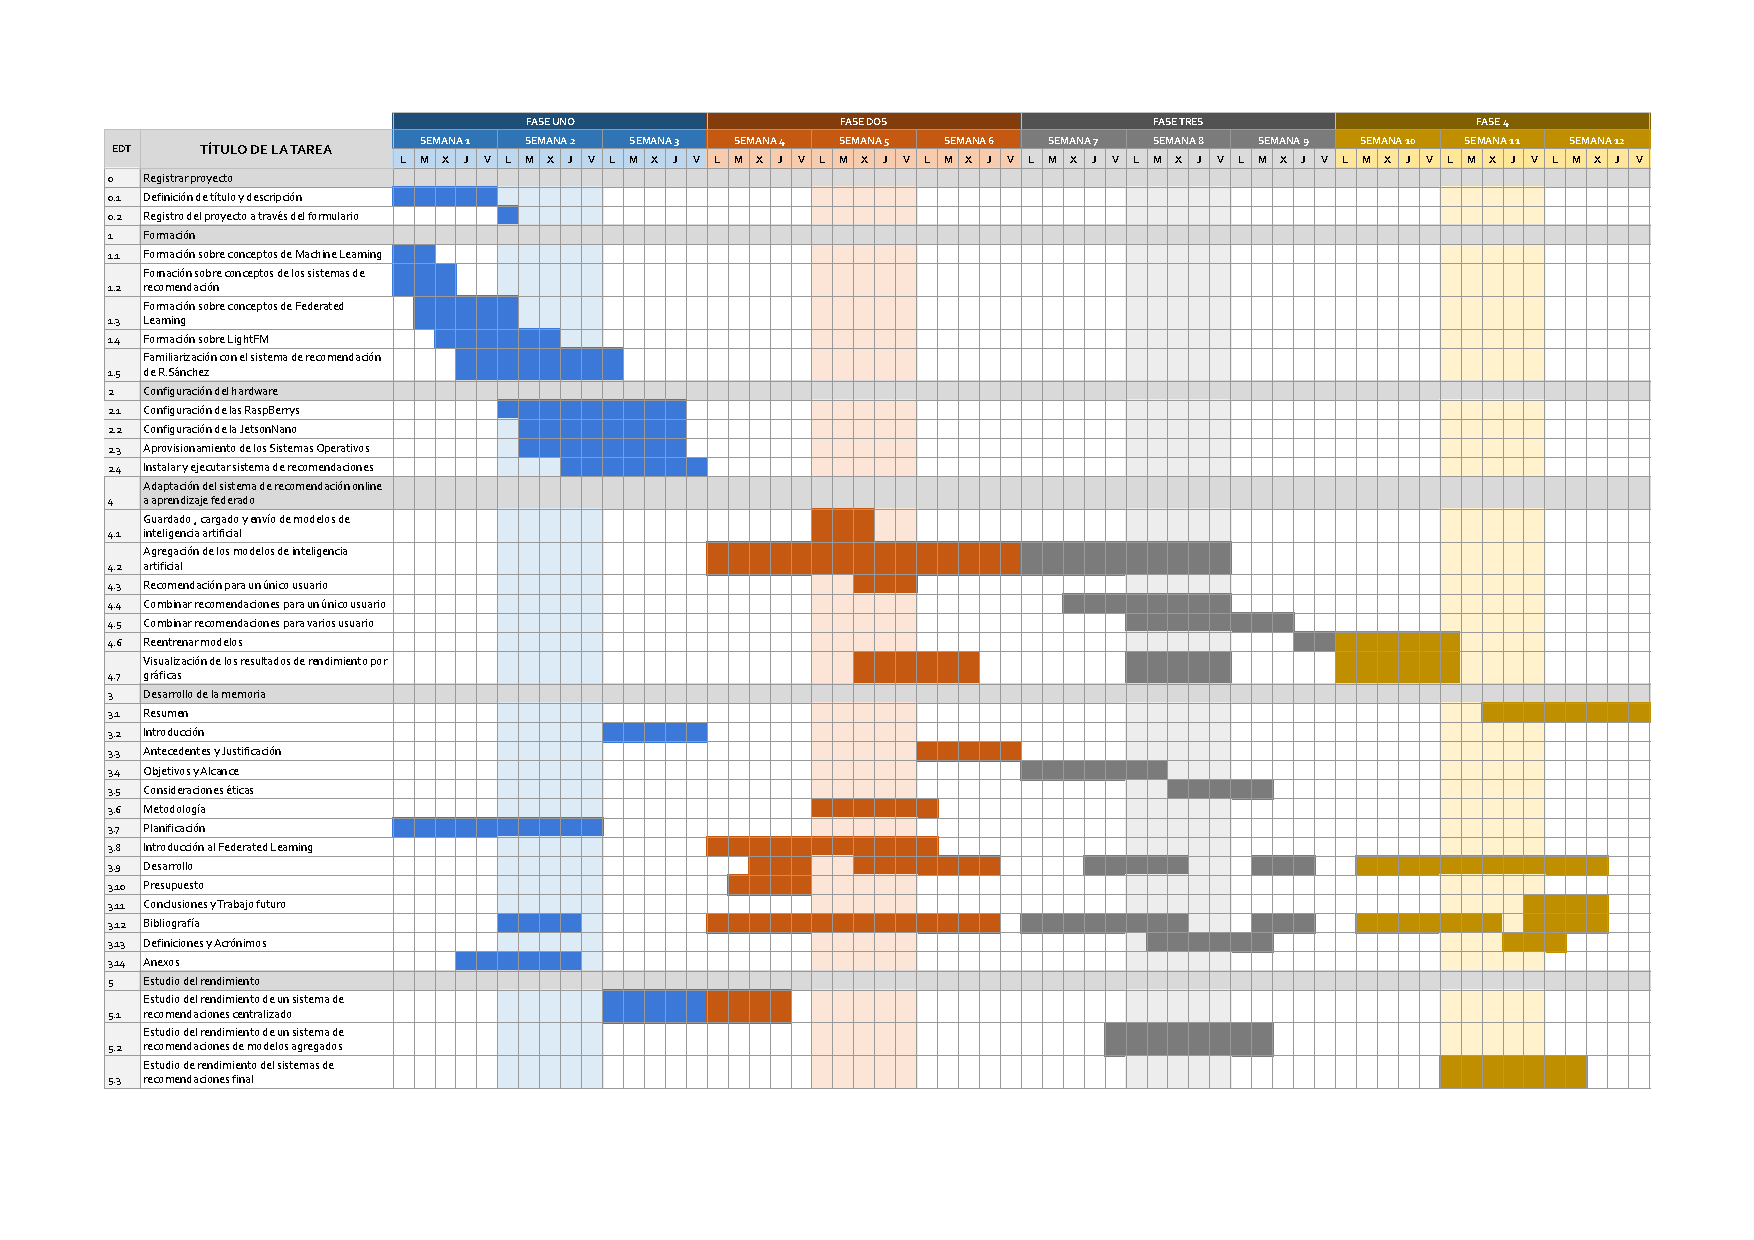
\includepdf[angle=90]{PDF/GanttPlanificacion}
    \caption{Planificación del proyecto}\label{table:planificacion}
\end{table}